\documentclass{article}
\usepackage[utf8]{inputenc}
\usepackage[spanish]{babel}
\usepackage{listingsutf8}
\usepackage{xcolor}
\usepackage{pdfpages}
\usepackage{geometry}
% to install algorithm2e pckg: sudo apt-get install texlive-science
\usepackage[ruled, vlined, nofillcomment]{algorithm2e}
\usepackage{float}
\usepackage{hyperref}
\usepackage{amsmath}
\usepackage{framed}
\usepackage[ruled, vlined, nofillcomment]{algorithm2e}

\geometry{
    a4paper,
    margin=1.2in
}

\title{75.29 - Teoría de Algoritmos I: Trabajo Práctico n. 2}
\author{
    \\\\\\\\
    \Large{Equipo Q:}\\
    Lavandeira, Lucas (\texttt{\#98042})\\\texttt{lucaslavandeira@gmail.com}\\
    \\
    Rozanec, Matias (\texttt{\#97404})\\\texttt{rozanecm@gmail.com}\\
    \\
    Sbruzzi, José (\texttt{\#97452})\\\texttt{jose.sbru@gmail.com}\\
    \\\\\\\\\\\\\\
}
\date{14.mayo.2018}

\begin{document}
\maketitle
\begin{figure}[!htp]
    \centering
    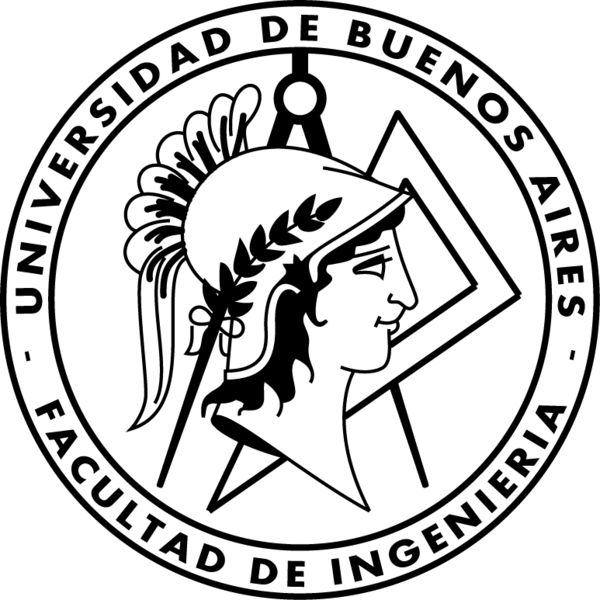
\includegraphics[scale=1]{res/fiuba_logo.png} 
\end{figure}
\begin{center}\normalsize{Facultad de Ingeniería, Universidad de Buenos Aires}\end{center}
\newpage

\tableofcontents
\newpage

% *** RESOLUCION ***
% Some settings for coding style
\lstset{
    basicstyle=\linespread{0.9}\ttfamily\footnotesize,
    frame=single,
    frameround=tttt,
    numbers=left,
    numberstyle=\tiny,
    linewidth=14cm,
    literate=
      {á}{{\'a}}1 {é}{{\'e}}1 {í}{{\'i}}1 {ó}{{\'o}}1 {ú}{{\'u}}1
      {Á}{{\'A}}1 {É}{{\'E}}1 {Í}{{\'I}}1 {Ó}{{\'O}}1 {Ú}{{\'U}}1
      {à}{{\`a}}1 {è}{{\`e}}1 {ì}{{\`i}}1 {ò}{{\`o}}1 {ù}{{\`u}}1
      {À}{{\`A}}1 {È}{{\'E}}1 {Ì}{{\`I}}1 {Ò}{{\`O}}1 {Ù}{{\`U}}1
      {ä}{{\"a}}1 {ë}{{\"e}}1 {ï}{{\"i}}1 {ö}{{\"o}}1 {ü}{{\"u}}1
      {Ä}{{\"A}}1 {Ë}{{\"E}}1 {Ï}{{\"I}}1 {Ö}{{\"O}}1 {Ü}{{\"U}}1
      {â}{{\^a}}1 {ê}{{\^e}}1 {î}{{\^i}}1 {ô}{{\^o}}1 {û}{{\^u}}1
      {Â}{{\^A}}1 {Ê}{{\^E}}1 {Î}{{\^I}}1 {Ô}{{\^O}}1 {Û}{{\^U}}1
      {œ}{{\oe}}1 {Œ}{{\OE}}1 {æ}{{\ae}}1 {Æ}{{\AE}}1 {ß}{{\ss}}1
      {ű}{{\H{u}}}1 {Ű}{{\H{U}}}1 {ő}{{\H{o}}}1 {Ő}{{\H{O}}}1
      {ç}{{\c c}}1 {Ç}{{\c C}}1 {ø}{{\o}}1 {å}{{\r a}}1 {Å}{{\r A}}1
      {€}{{\euro}}1 {£}{{\pounds}}1 {«}{{\guillemotleft}}1
      {»}{{\guillemotright}}1 {ñ}{{\~n}}1 {Ñ}{{\~N}}1 {¿}{{?`}}1
}




\part{Dinamico}
\section{Explicación del algoritmo}

\begin{algorithm}
\caption{mejoresPartidas(t,d)}
\KwData{Cantidad de turnos $t$ que demoran las partidas retornadas y disparos $d$ que se dispararán a continuación}
\KwResult{Partidas con menor cantidad de puntos obtenidas}
    $d \leftarrow \text{siguiente disparo}$ \\
    $t \leftarrow \text{turno actual}$ \\
    \If{$t=0$}{
        \KwRet{partida inicial sin disparos}
    }\Else{
        A $\leftarrow \bigcup_{d' \in D}$ mejoresPartidas$(t-1,d')$ \\
        A $\leftarrow$ conDisparo($d$,A) \\
        $p^* \leftarrow max_{a \in A}\left \{puntaje(a)\right \}$ \\
        A^* $\leftarrow \{ a \in A / puntaje(a)=p^*\}$ \\
        \KwRet{ A^* }
    }
\end{algorithm}

El algoritmo pretende devolver la lista de las mejores partidas posibles que se resuelvan en t turnos y que terminen con el disparo d, sin embargo, no lo logra. Devuelve las mejores partidas posibles al aplicarles el disparo d a cada una de las mejores partidas posibles en t-1 turnos.

En la implementación javascript, los hiperparámetros del algoritmo (es decir, el tablero, la cantidad de lanzaderas, la cantidad de barcos y los puntos de vida de cada uno) también se pasan como argumentos.

El algoritmo se construyó teniendo en cuenta la siguiente función de minimización:------------ TODO --------

\section{Calidad de heurística de Dinámico}

Dinamico no conforma un algoritmo de resolución de la situación planteada, sino una heurística. Esto se demuestra por medio del siguiente contraejemplo.

\begin{center}
\begin{tabular}{ c | c c c c c}
Hay una sola lanzadera.
\hline
V_i & t1 & t2 & t3 & t4 & t5
\hline
10    &  9 &  1 &  1 &  1 &  1 &  1 & 1 &  1 &  1 &  1 &  1 & 1  & 10 \\
1     &  1 &  1 &  1 &  1 &  1 &  1 & 1 &  1 &  1 &  1 &  1 & 1  & 10
\end{tabular}
\end{center}

En la solución mínima, el barco de vida 10 recibe un disparo en el primer turno, aprovechándose de esta forma el gran daño que puede recibir; y el puntaje alcanzado es 5. Sin embargo, debido a que Dinámico es una heurística que aplica un criterio de greedy para determinar la mejor decisión por turno, determina que la mejor decisión para el primer turno es la que lleve a un mejor puntaje, es decir, disparar al barco de salud 1 primero y al de salud 10 después. Así, el puntaje mínimo alcanzado por Dinámico será 11.

\section{Complejidad temporal del algoritmo}

El algoritmo Dinamico es memoizado. Como sus únicos parámetros son t y d, su complejidad temporal será lineal respecto de los valores que puede tomar cada uno de sus parámetros. En memoria, se generará una tabla como la siguiente:
\begin{center}
\begin{tabular}{c | c c c c}
turno & disparo posible 1 & disparo posible 2 & disparo posible 3 & ...
\hline
t_0 & & & & \\
t_1 & & & & \\
t_2 & & & & \\
t_3 & & & & \\
t_4 & & & & \\
t_5 & & & & \\
... & & & &
\end{tabular}
\end{center}
El costo añadido de computar la solución en cada "casilla" de la tabla es lineal al costo de obtener el puntaje de cada partida alternativa, y por lo tanto a la cantidad de partidas alternativas. Por otro lado, el costo de computar el puntaje de cada partida alternativa es lineal con la cantidad de barcos (ya que es necesario determinar si cada uno de ellos está vivo en la misma). Así, el costo del algoritmo memoizado para resolver mejoresPartidas(t,d)=O(t*disparos posibles*costo de cada casillero)=O(t*disparos posibles*disparos posibles*costo de obtener puntaje de una partida)=O(t*disparos posibles*disparos posibles*barcos)=O(t*disparos posibles^2*barcos) .

\section{Condiciones para que Dinámico sea óptimo}
Dinámico será óptimo cuando la mejor decisión posible en cada turno sea la que más barcos mate en ese turno. Esto sólo puede darse cuando las vulnerabilidades relacionadas a cada barco solamente ascienden a lo largo de la partida, cuando el tablero no es "rotatorio", tal como fue el planteo dado, es necesario asegurar también que ninguna partida dura tantos turnos como columnas del tablero. A continuación se demuestra esta afirmación para un tablero infinito, sin repeticiones.

\subsection{Planteo matemático de la hipótesis y demostración}

\subsubsection{Conceptos necesarios para expresar la hipótesis y la prueba}

Sea $v(t,b)$ la vulnerabilidad del barco $t$ en el turno $b$, con $t\geq0$ y $1\geq b \geq B$, siendo $B$ la cantidad de barcos.
Sea $d(t,b)$ una función tal que

\[
    d(t,b)=
    \begin{cases}
        1 & \text{si se dispara al barco $b$ en el turno $t$} \\
        0 & \text{en otro caso}
    \end{cases}
\]
Y sea $D$ el conjunto de todos los disparos $d$ que cumplen que:
$$ \sum_{b=1}^{B} d(t,b) = L  \forall t \geq 0 $$

Sea $h_{d,v} (t,b)$ una función que representa la salud del barco $b$ en el turno $t$, al usar los disparos $d$ y las vulnerabilidades $v$:
\[
    h_{d,v}(t,b)=
    \begin{cases}
        h(t-1,b)-v(t,b) \cdot d(t,b) & \text{si $t>0$} \\
        V_b & \text{si t=0}
    \end{cases}
\]
Siendo $V_b$ la salud inicial de cada barco. Sea $H_{d,v}(b,t)$ una función que indica si el barco $b$ vive en el turno $t$, usando los disparos $d$ y las vulnerabilidades $v$.
\[
    H_{d,v}(t,b)=
    \begin{cases}
        1 & \text{si $h_{d,v}(t,b)>0$} \\
        0 & \text{en caso contrario}
    \end{cases}
\]

Y sea también $H_{d,v}(t)$ tal que: $$H_{d,v}(t)=\sum_{b=1}^{B} H_{d,v}(t,b)$$

Sea la función $G(d,v,t)$ que indica si en el turno $t$, el disparo $d$ representa una formado por medio de la estrategia greedy, que consiste en elegir el disparo que destruya más barcos:
\[
    G(d,v,t)=
    \begin{cases}
        1 & \text{si $h_{d,v}(t)=min_{d' \in D} \left \{ H_{d',v}(t) \right \} $} \\
        0 & \text{si no}
    \end{cases}
\]

Sea la función $G*(d,v,t)$ que representa si los disparos de todos los turnos hasta $t$ fueron greedy:
\[
    G^*(d,v,t)=
    \begin{cases}
        G(d,v,t) \cdot G^*(d,v,t-1) & \text{si $T>0$} \\
        1 & \text{si $T=0$}
    \end{cases}
\]

Sea la función $P_{d,v}(t)$ la cantidad de puntos acumulados hastael turno $t$ al usar el disparo $d$ y las vulnerabilidades $v$:
\[
    P_{d,v}(t)=
    \begin{cases}
        H_{d,v}(t) + P_{d,v}(t-1) & \text{si $t>0$} \\
        0 & \text{si $t=0$}
    \end{cases}
\]


\subsubsection{Hipótesis}
\begin{framed}
Para cualquier $T$ natural mayor a 0 se cumple que: \newline
Dado $v$ tal que: 
$$ v(t+1,b) 
\geq 
v(t,b) \forall 0 \leq t \leq T, 1 \leq b \leq B $$
Y dado $d$ tal que: $$G^*(d,v,T)=1$$
Entonces: $$P_{d,v}(T)=min_{d' \in D} \left \{ P_{d',v}(T) \right \}$$
\end{framed}

\subsubsection{Demostración: caso base}
Para $T=0$ la hipótesis es verdadera porque $P_{d,v}(T)=0 \forall d,v$.


\subsubsection{Planteo del caso inductivo}
Para $T > 0$, tenemos que se cumple para $T-1$ que:
\begin{framed}
Dado $v$ tal que: $$ v(t+1,b) \geq v(t,b) \forall 0 \leq t \leq T-1, 1 \leq b \leq B $$
Y dado $d$ tal que: $$G^*(d,v,T-1)=1$$
Entonces: $$P_{d,v}(T-1)=min_{d' \in D} \left \{ P_{d',v}(T-1) \right \}$$
\end{framed}
A partir de esa proposición, queremos probar que teniendo:
\begin{framed}
Dado $v$ tal que: $$ v(t+1,b) \geq v(t,b) \forall 0 \leq t \leq T, 1 \leq b \leq B $$
Y dado $d$ tal que: $$G^*(d,v,T)=1$$
\end{framed}
Podemos concluir que: $$P_{d,v}(T)=min_{d' \in D} \left \{ P_{d',v}(T) \right \}$$

\subsubsection{Demostración del caso inductivo}
Por la definición de $P$: $$P_{d,v}(T)=H_{d,v}(T)+P_{d,v}(T-1)$$
Por la hipótesis inductiva, que afirma que $P_{d,v}(T-1)=min_{d^* \in D}\left \{ P_{d^*,v}(T-1) \right \}$ podemos definir que:
$$P_{d,v}(T)=H_{d,v}(T)+min_{d^* \in D}\left \{ P_{d^*,v}(T-1) \right \}$$

Debido a que: $$G^*(d,v,T)=1 \Rightarrow G(d,v,T)=1 \Rightarrow H_{d,v}(T)=min_{d' \in D} \left \{ H_{d',v}(T) \right \}$$
Podemos concluir, combinando estas últimas dos proposiciones, que:
$$P_{d,v}(T)=min_{d' \in D} \left \{ H_{d',v}(T) \right \}+min_{d^* \in D}\left \{ P_{d^*,v}(T-1) \right \}$$

Una manera alternativa de definir $P_{d,v}(t)$ es:$$P_{d,v}(t)=\sum_{i=1}^{t} H_{d,v}(i)$$

Agregando esta definición a la proposición anterior tenemos que:

$$P_{d,v}(T)=min_{d' \in D} \left \{ H_{d',v}(T) \right \}+min_{d^* \in D}\left \{ \sum_{i=1}^{T-1} H_{d^*,v}(i) \right \}$$
Debido a que los disparos $d$ en cada uno de los turnos son independientes, y la minimización tiene en cuenta sólo la efectividad de cada turno:
$$P_{d,v}(T)=min_{d' \in D} \left \{ H_{d',v}(T) \right \}+\sum_{i=1}^{T-1} min_{d^* \in D}\left \{  H_{d^*,v}(i) \right \}$$

$$P_{d,v}(T)=\sum_{i=1}^{T} min_{d^* \in D}\left \{  H_{d^*,v}(i) \right \}$$

Teniendo en cuenta la independencia de los disparos en cada uno de los turnos citada anteriormente, consecuencia de la condición impuesta sobre $v$, que implica que cualquier barco que podría haber sido destruído en cierto turno puede ser destruído en el siguiente, podemos concluir que:
$$P_{d,v}(T)=min_{d'' \in D}\left \{ \sum_{i=1}^{T} H_{d'',v}(i) \right \}$$
Lo cual concluye la demostración.

